\documentclass{article}
\usepackage{amsmath, amsthm, amssymb}
\usepackage{tikz}
\usepackage{array}
\usepackage{mathtools}
\usepackage{graphicx}

\begin{document}
\section*{\huge Homework Sheet 2}
\begin{flushright}
   \textbf{Author: Abdullah Oğuz Topçuoğlu}
\end{flushright}

% Mathematics for Computer Scientists III
% Exercise Sheet 2
% Exercise 5 (4 Points)
% Let the function f : R2 → R be defined by
% f(x1, x2) := |x1| + |x2|.
% At which points (x0
% 1, x0
% 2) ∈ R2 is f partially differentiable? Determine the partial derivatives of f
% at the points (x0
% 1, x0
% 2) ∈ R2 at which f is partially differentiable.
% Exercise 6 (4 Points)
% Let D := {(x1, x2) ∈ R2 : x1 ∕= x2
% 2, x2 > 0} and f : D → R a function defined by
% f(x1, x2) := x1 ln(x2)
% (x1 − x2
% 2)x2
% .
% (i) Explain why D is open.
% (ii) Show that f is partially differentiable and determine the partial derivatives at any point
% (x0
% 1, x0
% 2) ∈ D.
% (iii) Determine the gradient of f at any point (x0
% 1, x0
% 2) ∈ D.
% Exercise 7 (4 Points)
% Let f : R2 → R be a function defined by
% f(x1, x2) :=
% 󰀫
% (x2
% 1 + x2
% 2)sin
% 󰀓 1
% x2
% 1+x2
% 2
% 󰀔
% , (x1, x2) ∕= (0, 0)
% 0 , (x1, x2) = (0, 0) .
% (i) Show that f is partially differentiable.
% (ii) Show that f is totally differentiable at the point (0, 0). Hint: Use 1.7.2 and 1.7.3.
% (iii) Show that f is not continuously differentiable at the point (0, 0).
% Exercise 8 (4 Points)
% Let f : R2 → R be a function defined by
% f(x1, x2) :=
% 󰀫 x1x3
% 2−x3
% 1x2
% x2
% 1+x2
% 2
% , (x1, x2) ∕= (0, 0)
% 0 , (x1, x2) = (0, 0) .
% (i) Show that f is twice continuously differentiable at any point x = (x1, x2) ∈ R2 \ {(0, 0)} and
% determine the Hessian matrix of f at x.
% (ii) Show that f is twice partially differentiable at point (0, 0) and determine the Hessian matrix
% of f at (0, 0). Why does the form of the Hessian matrix not contradict Schwarz’s theorem
% (Theorem 1.5.12)?

\section*{Problem 5}

We are given the function
\[
   f(x_1, x_2) := |x_1| + |x_2|.
\]

We are looking for points \(x^0 \in \mathbb{R}^2\) where \(\frac{\partial f}{\partial x^0_1}\) and \(\frac{\partial f}{\partial x^0_2}\) exist.
First things first that we realize the function is symmetric in both variables, so we can just focus on one of them and the other will follow the same logic. \\
Let's consider the partial derivative with respect to \(x^0_1\):
\begin{align*}
   \frac{\partial f}{\partial x^0_1} &= \lim_{h \to 0} \frac{f(x^0_1 + h, x^0_2) - f(x^0_1, x^0_2)}{h}. \\
   &= \lim_{h \to 0} \frac{|x^0_1 + h| + |x^0_2| - (|x^0_1| + |x^0_2|)}{h}. \\
   &= \lim_{h \to 0} \frac{|x^0_1 + h| - |x^0_1|}{h}.
\end{align*}
Now we have to consider different cases for \(x^0_1\):
\begin{itemize}
   \item If \(x^0_1 > 0\):
   \begin{align*}
      \frac{\partial f}{\partial x^0_1} &= \lim_{h \to 0} \frac{(x^0_1 + h) - x^0_1}{h} = \lim_{h \to 0} \frac{h}{h} = 1.
   \end{align*}
   \item If \(x^0_1 < 0\):
   \begin{align*}
      \frac{\partial f}{\partial x^0_1} &= \lim_{h \to 0} \frac{-(x^0_1 + h) + x^0_1}{h} = \lim_{h \to 0} \frac{-h}{h} = -1.
   \end{align*}
   \item If \(x^0_1 = 0\):
   \begin{align*}
      \frac{\partial f}{\partial x^0_1} &= \lim_{h \to 0^+} \frac{|h| - 0}{h} = \lim_{h \to 0^+} \frac{h}{h} = 1, \\
      \frac{\partial f}{\partial x^0_1} &= \lim_{h \to 0^-} \frac{|-h| - 0}{h} = \lim_{h \to 0^-} \frac{-h}{h} = -1.
   \end{align*}
   Since the left-hand limit and right-hand limit are not equal, the partial derivative does not exist at this point.
\end{itemize}

So partial derivates exist for all points where \(x^0_1 \neq 0\). By symmetry, the same applies for \(x^0_2\). \\
\textbf{Partial Derivaties:}
\begin{align*}
   \frac{\partial f}{\partial x^0_1} =
   \begin{cases}
      1, & x^0_1 > 0 \\
      -1, & x^0_1 < 0
   \end{cases}, \\
   \frac{\partial f}{\partial x^0_2} =
   \begin{cases}
      1, & x^0_2 > 0 \\
      -1, & x^0_2 < 0
   \end{cases}
\end{align*}

\section*{Problem 6}
We are given the set
\begin{align*}
   D := \{(x_1, x_2) \in \mathbb{R}^2 : x_1 \neq x_2^2, x_2 > 0\}
\end{align*}

and the function
\begin{align*}
   f : D \to \mathbb{R}, \quad f(x_1, x_2) := \frac{x_1 \ln(x_2)}{(x_1 - x_2^2)x_2}.
\end{align*}

\subsection*{(i)}
We need to show that for any point \(x \in D\) we can find an open ball around it. \\

\begin{figure}[h!]
  \centering
  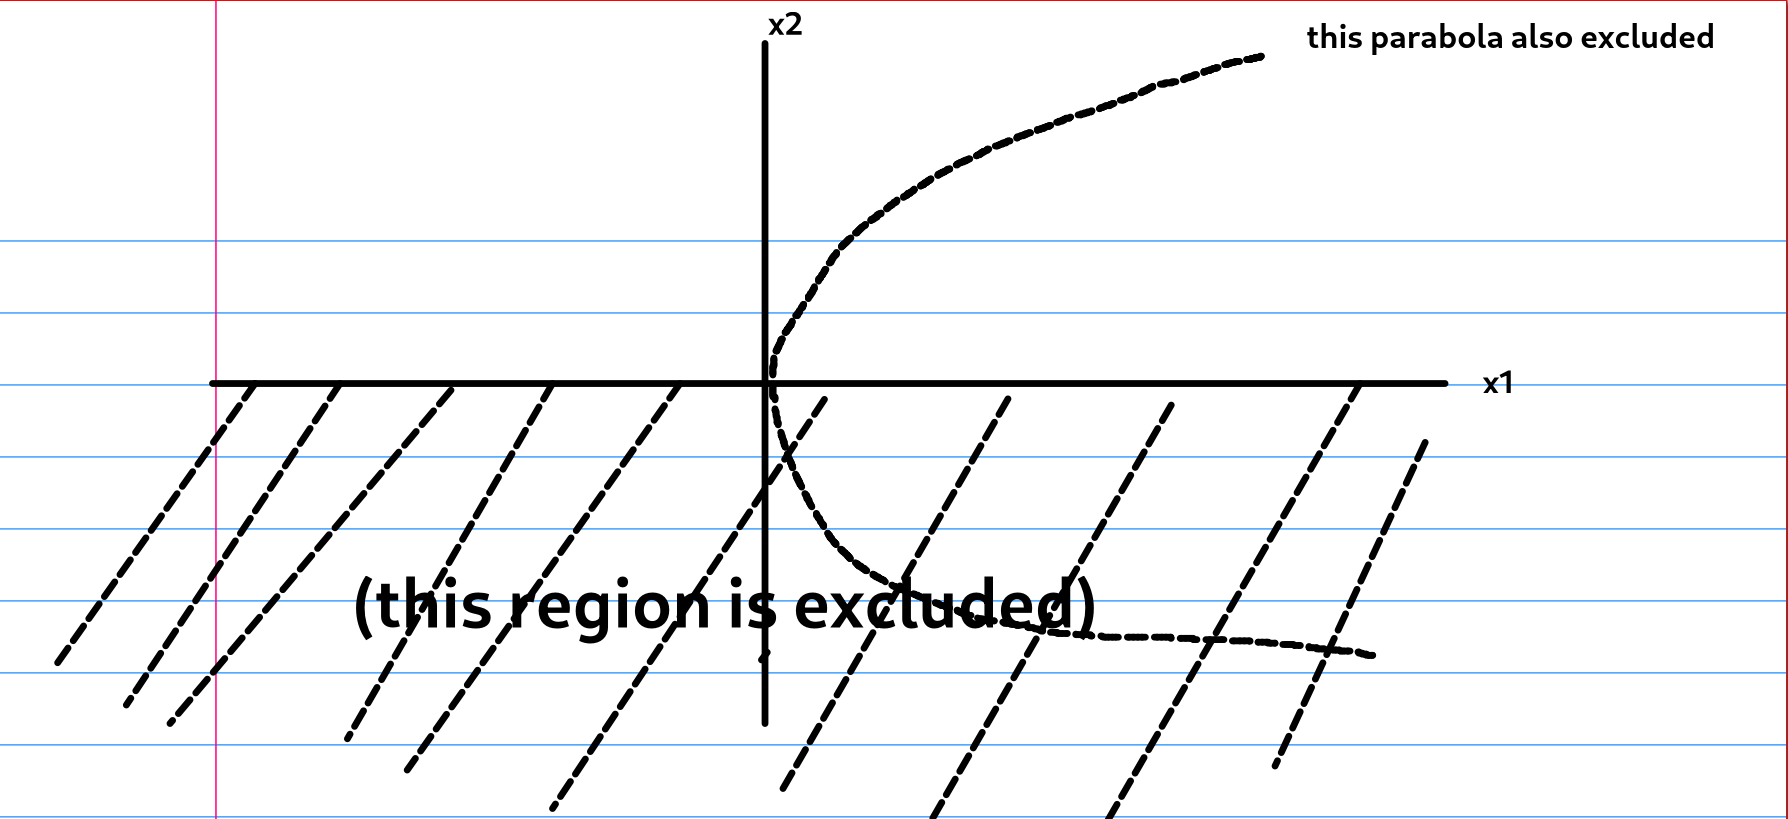
\includegraphics[width=\linewidth]{Screenshot From 2025-10-22 12-07-40.png}
  \caption{The set D}
\end{figure}

So if we pick a poitn in \(D\) we can get the distance to \(x_1\) axis and distance to the parabola in the image and if we choose the radius of the open ball to be
the smaller of both then every point in that open ball will be in \(D\) because we are guaranteed to not touch the \(x_1\) axis and the parabola. \\
Thats why \(D\) is open.

\end{document}